% Template Source: This template has been downloaded from:
% http://www.latextemplates.com/template/stylish-article
% Changed by Jelle Spijker and especcialy adapted for the
% Univeristy of applied Sciences HAN (spijker.jelle@gmail.com)
% License: CC BY-NC-SA 3.0 
%%%%%%%%%%%%%%%%%%%%%%%%%%%%%%%%%%%%%%%%%

%----------------------------------------------------------------------------------------
%	PACKAGES AND OTHER DOCUMENT CONFIGURATIONS
%----------------------------------------------------------------------------------------

\documentclass[fleqn,10pt]{SelfArx} % Document font size and equations flushed left

\usepackage{lipsum} % Required to insert dummy text. To be removed otherwise
\usepackage{animate}
\usepackage[style=numeric,citestyle=numeric,sorting=nyt,sortcites=true,autopunct=true,babel=hyphen,hyperref=true,abbreviate=false,backref=true,backend=bibtex]{biblatex}
\addbibresource{../bib/bib.bib} % BibTeX bibliography file
%----------------------------------------------------------------------------------------
%	HAN Variable
%----------------------------------------------------------------------------------------
\newcommand{\instutionname}{HAN University of Applied Sciences}
\newcommand{\degree}{Bachelor}
\newcommand{\studentnr}{495653}
\newcommand{\mti}{IHC MTI B.V. }
\newcommand{\vsa}{vision based sand analyzer}
\newcommand{\ihc}{Royal IHC }
\newcommand{\evd}{embedded vision design }
\newcommand{\wtb}{mechanical engineering }

%----------------------------------------------------------------------------------------
%	COLUMNS
%----------------------------------------------------------------------------------------

\setlength{\columnsep}{0.55cm} % Distance between the two columns of text
\setlength{\fboxrule}{0.75pt} % Width of the border around the abstract

%----------------------------------------------------------------------------------------
%	COLORS
%----------------------------------------------------------------------------------------

\definecolor{color1}{RGB}{0,0,90} % Color of the article title and sections
\definecolor{color2}{RGB}{0,20,20} % Color of the boxes behind the abstract and headings

%----------------------------------------------------------------------------------------
%	HYPERLINKS
%----------------------------------------------------------------------------------------

\usepackage{hyperref} % Required for hyperlinks
\hypersetup{hidelinks,colorlinks,breaklinks=true,urlcolor=color2,citecolor=color1,linkcolor=color1,bookmarksopen=false,pdftitle={Title},pdfauthor={Author}}

%----------------------------------------------------------------------------------------
%	ARTICLE INFORMATION
%----------------------------------------------------------------------------------------

\JournalInfo{\instutionname, Stage2, Period 2015-2016} % Journal information
\Archive{} % Additional notes (e.g. copyright, DOI, review/research article)

\PaperTitle{A proposal to use Github as PDM environment for a \vsa} % Article title

\Authors{Jelle Spijker\textsuperscript{1}* \studentnr} % Authors
\affiliation{\textsuperscript{1}\textit{Department of Engineering, HAN University of Applied Sciences, Arnhem, the Netherlands}} % Author affiliation
\affiliation{*\textbf{Corresponding author}: \href{mailto:spijker.jelle@gmail.com}{spijker.jelle@gmail.com}} % Corresponding author

\Keywords{Product Data Management --- Vision Soil Analyzer --- Github} % Keywords - if you don't want any simply remove all the text between the curly brackets
\newcommand{\keywordname}{Keywords} % Defines the keywords heading name

%----------------------------------------------------------------------------------------
%	ABSTRACT
%----------------------------------------------------------------------------------------

\Abstract{\lipsum[1]~}

%----------------------------------------------------------------------------------------

\begin{document}

\flushbottom % Makes all text pages the same height

\maketitle % Print the title and abstract box

\tableofcontents % Print the contents section

\thispagestyle{empty} % Removes page numbering from the first page

%----------------------------------------------------------------------------------------
%	ARTICLE CONTENTS
%----------------------------------------------------------------------------------------

\section*{Introduction} % The \section*{} command stops section numbering

\addcontentsline{toc}{section}{Introduction} % Adds this section to the table of contents
This article proposes a setup for a PDM\footnote{Product Data Management} environment used during developed of a \vsa\footnote{Working title VSA}. This new line of product(s) is currently being developed at \mti and has the ability to analyze sand by its optical characteristics. 

The concept and initial design of this product finds it origin at the minor \evd and will be further developed during the graduation phase \wtb at the HAN. Design and production of this product leans on the following three disciplines: mechanical, electrical and software engineering. Due to its multidisciplinary properties it is relevant to implement a PDM environment which acts as a solid basis for all disciplines and allows for interaction and flexibility.

\mti is a R\&D based company and subsidiary of \ihc. Although \ihc is currently in the process of implementing a new PDM and ERP\footnote{Enterprise Resource Planning} environment named IHC ONE, linking all wharfs, departments and subsidiary companies using Siemens Teamcenter and IFS. Current data systems are all still folder and DMS\footnote{Document Management System} based. This setup doesn't allow for the necessary flexibility and revision controlled, that is needed for the VSA project.

It is therefore proposed to make use of Github as an PDM environment. Github is a web-based Git\footnote{version control system for software development designed and developed by Linus Torvalds and used for the Linux Kernels} repository, used in the development of software and build upon the principles of collaboration. Due to the origins in software development this environment is largely unknown in the mechanical engineering branch. But it is gaining traction as an PDM environment according \citeauthor{oleg_github_2013}\cite{oleg_github_2013}. 

Because Github is strongly rooted in software development there is an excellent revision control


%------------------------------------------------

\section{Vision based Sand Analyzer}

\subsection{Product breakdown}

\subsection{The toolboxes}

\subsubsection{Software engineering}

\subsubsection{Electrical engineering}

\subsubsection{Mechanical engineering}

\section{Github}

\subsection{Workflow}

\subsubsection{Software disciplines}

\subsubsection{Electrical engineering}

\subsubsection{Mechanical engineering}

\begin{figure*}[ht]\centering % Using \begin{figure*} makes the figure take up the entire width of the page
%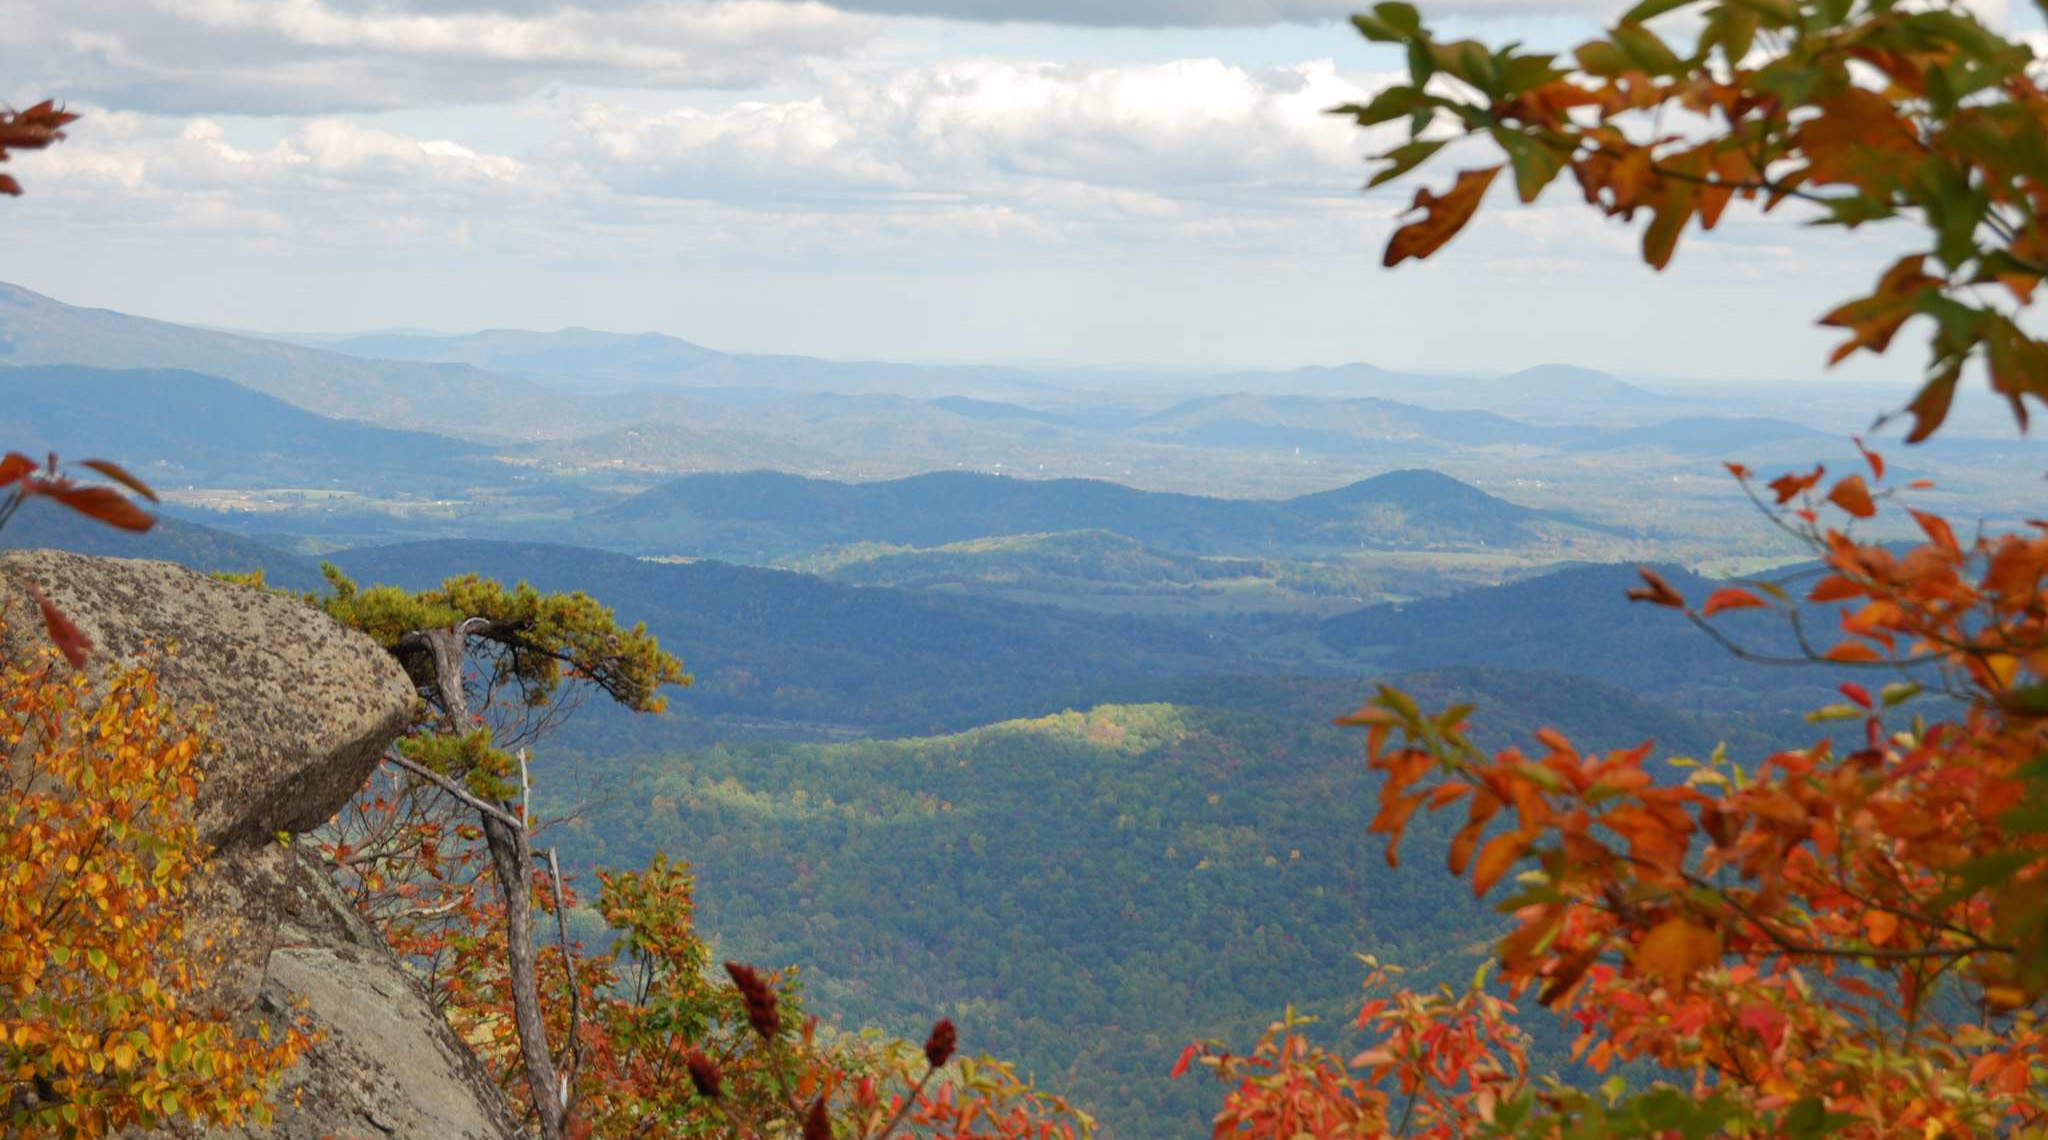
\includegraphics[width=\linewidth]{view}
\animategraphics[loop,autoplay]{12}{../images/githubframe-}{0}{34}
\caption{Revision control of 3D models, source: \citeauthor{skalnik_3d_2013}\cite{skalnik_3d_2013}}
\label{fig:view}
\end{figure*}

\lipsum[4] % Dummy text

\begin{equation}
\cos^3 \theta =\frac{1}{4}\cos\theta+\frac{3}{4}\cos 3\theta
\label{eq:refname2}
\end{equation}

\lipsum[5] % Dummy text

\begin{enumerate}[noitemsep] % [noitemsep] removes whitespace between the items for a compact look
\item First item in a list
\item Second item in a list
\item Third item in a list
\end{enumerate}

\subsection{Subsection}

\lipsum[6] % Dummy text

\paragraph{Paragraph} \lipsum[7] % Dummy text
\paragraph{Paragraph} \lipsum[8] % Dummy text

\subsection{Subsection}

\lipsum[9] % Dummy text

\begin{figure}[ht]\centering
\caption{In-text Picture}
\label{fig:results}
\end{figure}

Reference to Figure \ref{fig:results}.

%------------------------------------------------

\section{Results and Discussion}

\lipsum[10] % Dummy text

\subsection{Subsection}

\lipsum[11] % Dummy text

\begin{table}[hbt]
\caption{Table of Grades}
\centering
\begin{tabular}{llr}
\toprule
\multicolumn{2}{c}{Name} \\
\cmidrule(r){1-2}
First name & Last Name & Grade \\
\midrule
John & Doe & $7.5$ \\
Richard & Miles & $2$ \\
\bottomrule
\end{tabular}
\label{tab:label}
\end{table}

\subsubsection{Subsubsection}

\lipsum[12] % Dummy text

\begin{description}
\item[Word] Definition
\item[Concept] Explanation
\item[Idea] Text
\end{description}

\subsubsection{Subsubsection}

\lipsum[13] % Dummy text

\begin{itemize}[noitemsep] % [noitemsep] removes whitespace between the items for a compact look
\item First item in a list
\item Second item in a list
\item Third item in a list
\end{itemize}

\subsubsection{Subsubsection}

\lipsum[14] % Dummy text

\subsection{Subsection}

\lipsum[15-23] % Dummy text

%------------------------------------------------
\phantomsection
\section*{Acknowledgments} % The \section*{} command stops section numbering

\addcontentsline{toc}{section}{Acknowledgments} % Adds this section to the table of contents

So long and thanks for all the fish.

%----------------------------------------------------------------------------------------
%	REFERENCE LIST
%----------------------------------------------------------------------------------------
\phantomsection
\printbibliography

%----------------------------------------------------------------------------------------

\end{document}